%\documentclass[preprint,tightenlines,showpacs,showkeys,floatfix,
%nofootinbib,superscriptaddress,fleqn]{revtex4} 
\documentclass[APS,floatfix,nofootinbib,superscriptaddress,fleqn,preprint]{revtex4} 
%\documentclass[aps,epsfig,tightlines,fleqn]{revtex4}
\usepackage[utf]{kotex}
\usepackage[HWP]{dhucs-interword}
\usepackage[dvips]{color}
\usepackage{graphicx}
\usepackage{bm}
%\usepackage{fancyhdr}
%\usepackage{dcolumn}
\usepackage{defcolor}
\usepackage{amsmath}
\usepackage{amsfonts}
\usepackage{amssymb}
\usepackage{amscd}
\usepackage{amsthm}
\usepackage[utf8]{inputenc}
 \usepackage{setspace}
%\pagestyle{fancy}

\begin{document}

\title{\Large 2022년 1학기 물리학 I: Quiz 2}
\author{Hui-Jae Lee} 
\email{hjlee6674@inha.edu}
\author{김현철\footnote{Office: 5S-436D (면담시간 매주s
    화요일-16:00$\sim$20:00)}} 
\email{hchkim@inha.ac.kr}
\affiliation{Hadron Theory Group, Department of Physics, Inha University,
Incheon 22212, Republic of Korea }
\date{Spring semester, 2022}


\vspace{1.cm}
\begin{abstract}
\noindent \textbf{ {\color{red}주의}: \color{blue} 단 한 번의 부정행위도 절대
  용납하지 않습니다. 적발 시, 학점은 F를 받게 됨은 물론이고,
  징계위원회에 회부합니다. One strike out임을 명심하세요.}\\
\\
문제는 다음 쪽부터 나옵니다.  \\ \\
{\bf Date:} 2022년 3월 7일 (월) 15:30-16:15 
\\
{\bf 학번:} \hspace{4cm}
{\bf 이름:} 

\end{abstract}
\maketitle

\noindent {\bf 문제 1 [20pt]}
그림~\ref{fig:1}과 같이 크기가 각각 1, 2, 4인 세 벡터 $\vec{A}$,
$\vec{B}$, $\vec{C}$가 같은 평면상에 놓여 있다. 벡터 $\vec{A}$와 벡터
$\vec{B}$는 서로 수직이고, 벡터 $\vec{B}$와 벡터 $\vec{C}$의 끼인각이 30°일 때,
벡터 $\vec{C}$는 벡터 $\vec{A}$와 벡터 $\vec{B}$를 사용하여
\begin{align*}
\vec{C} = \alpha \vec{A} + \beta\vec{B}  
\end{align*}
로 나타낼 수 있다. 두 상수 $\alpha$와 $\beta$를 구하여라. 
\begin{figure}[ht]
  \centering
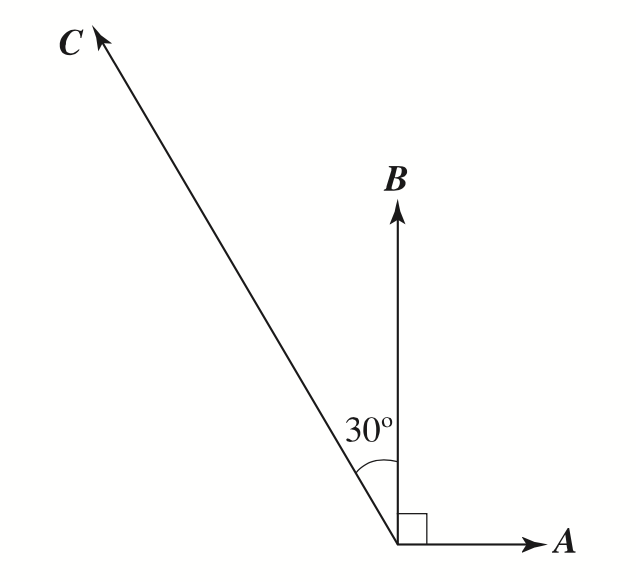
\includegraphics[scale=0.6]{Qfig3-1-20220307.png}  
  \caption{문제 1}
  \label{fig:1}
\end{figure} 

\noindent {\bf 해답} $\vec{A}$ 와 $\vec{B}$ 가 서로 수직이므로,
$\vec{A} \cdot \vec{B} =0 $ 이다. 이는 다음을 의미한다. 
\begin{align*}
  \vec{C} \cdot \vec{A} &=
 \alpha(\vec{A}\cdot\vec{A}) + \beta(\vec{B}\cdot\vec{A})
   = \alpha|\vec{A}|^2=\alpha \\ 
  \vec{C} \cdot \vec{B} &= \alpha(\vec{A}\cdot\vec{B}) +
                          \beta(\vec{B}\cdot\vec{B})
                          =\beta|\vec{B}|^2=4\beta  
\end{align*}
스칼라곱의 정의를 이용하면 $\alpha$ 와 $\beta$ 를 구할 수
있다. 스칼라곱의 정의는 다음과 같다. 
\begin{align*}
  \vec{a} \cdot \vec{b} = |\vec{a}||\vec{b}|\cos{\theta}
\end{align*}
이로부터 $\alpha$ 와 $\beta$ 는 다음과 같이 표현이 가능하다.
\begin{align*}
  \alpha &= \vec{C} \cdot \vec{A} =|\vec{C}||\vec{A}|\cos{120^{\circ}}
           = (4) (1) \left(-\frac{1}{2}\right) = -2 \\ 
  4\beta &= \vec{C} \cdot \vec{B} =|\vec{C}||\vec{B}|\cos{30^{\circ}}
           = (4) (2)\left(\frac{\sqrt{3}}{2}\right) = 4\sqrt{3} 
\end{align*}
따라서, $\alpha = -2$, $\beta = \sqrt{3}$ 이고 $\vec{C}$ 는 다음과 같다.
\begin{align*}
  \vec{C} = -2 \vec{A} + \sqrt{3} \vec{B}
\end{align*}
\vspace{0.5cm}

\noindent {\bf 문제 2 [10pt]}
물리학자이자 의사였던 미공군 존 스탭(John P. Stapp) 대령은 제트기에서
조정사가 비상탈출을 했을 때 살아남을 수 있는지 직접 실험을
했다. 1954년 3월 19일, 그는 로켓을 단 차를 선로 위를 달릴 수 있도록
제작한 뒤,  1\,011 km/h의 속력으로 달렸다. 그리고 도착점에 거의 다
도달했을 때, 제동을 걸어 1.40 s만에 멈췄다. 
\begin{figure}[htp]
  \centering
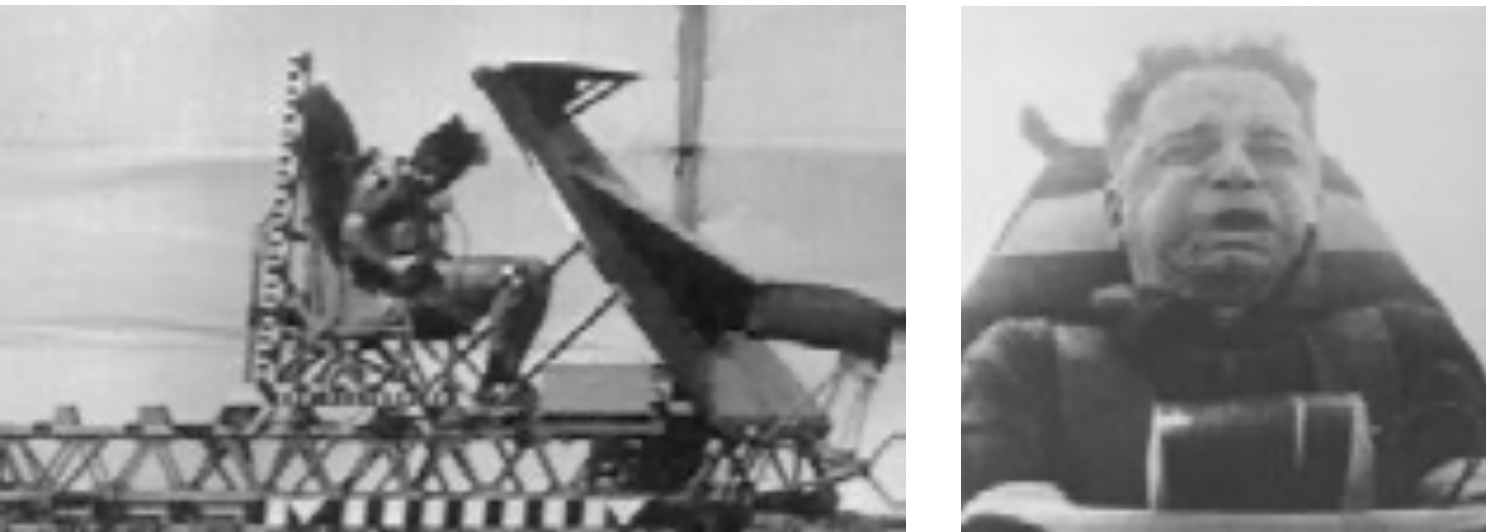
\includegraphics[scale=0.5]{Qfig3-2-20220307.png}  
  \caption{문제 2}
  \label{fig:2}
\end{figure}
\begin{itemize}
\item[(가)] 스탭 대령이 경험한 음의 가속도(감속도)를 구하여라. 구한
  가속도의 크기를 중력가속도 $g=9.80\,\mathrm{m/s^2}$로 나타내어라.
\item[(나)] 이 가속도를 받는 1.40 s  동안 스탭 대령이 간 거리는 얼마인가?
\end{itemize}
(이 실험으로 스탭 대령은 무릎뼈가 골절되고, 눈에 심각한 부상을 입어서
훗날 백내장으로 고생했다고 한다. 이 실험으로 스탭 대령은 자동차에 안전벨트를
도입하는 데 지대한 공을 세웠다.) \\
\noindent {\bf 풀이} 
(가) 스탭 대령의 처음 속력은 1\,011 km/h 이고
    정지하였으므로, 나중 속력은 0 km/h 이다. 걸린 시간 1.40 s 와 단위
    환산을 고려하여 다음과 같이 평균 가속도를 계산할 수 있다. 
  \begin{align}
    a_{\mathrm{avg}} &= \frac{v_f-v_i}{t_f-t_i} =
              \frac{(0-1\,011)\,\mathrm{km/h}}{(1.40-0)\,\mathrm{s}} \cr
              &= -\left(\frac{(722.143\,\mathrm{km/s})}{1\,\mathrm{h}} \right)
                \left( \frac{1\,000\,\mathrm{s}}{1\,\mathrm{km}}\right)
                \left(\frac{1\,\mathrm{h}}{3\,600\,\mathrm{s}}\right)
                = - (2.01\times 10^2)\,\mathrm{m/s^2}
  \end{align} 
  이 된다. 따라서 평균가속도의 크기는 
  \begin{align*}
|a_{\mathrm{avg}}| =  (2.01\times 10^2)\,\mathrm{m/s^2}   
  \end{align*}
이 된다. 

\noindent  중력 가속도의 크기를 $g$ 라고 하면, 평균가속도의 크기는 
  \begin{align}
   a_{\mathrm{avg}} =  \left(\mathrm{201\,m/s^2}\right)
    \left(\frac{1\,g}{9.80\,\mathrm{m/s^2}}\right)
    = 20.5 \,g
  \end{align} 
  스탭 대령은 감속하면서 중력 가속도의 크기의 약 20.5배에 달하는 가속도를 받았다.
  \\
  \\
\noindent (나) 처음 속력과 나중 속력, 평균 가속도를 알고 있으므로,
    다음의 공식을 이용해 이동한 거리를 구할 수 있다. 
  \begin{align}
    v^2=v_0^2+2a_{\mathrm{avg}}(x-x_0)
  \end{align}
  여기서 $v_0$는
  \begin{align*}
    v_0 = (1\,011\,\mathrm{km/h}) \left(
    \frac{1\,000\,\mathrm{s}}{1\,\mathrm{km}}\right) 
    \left(\frac{1\,\mathrm{h}}{3\,600\,\mathrm{s}}\right)
    =280.8\,\mathrm{m/s}
  \end{align*}
  이다. 따라서 $x-x_0$는 
  \begin{align*}
x-x_0 =   \frac{v^2-v_0^2}{2a_{\mathrm{avg}}} =
    \frac{-(280.8)^2\,\mathrm{m^2/s^2}}{2(-201)\,\mathrm{m/s^2}}
   = 1.96\times 10^2\,\mathrm{m} 
 \end{align*}
이동하였다. 
\vspace{0.5cm}

\noindent {\bf 문제 3 [10pt]} 
어떤 전투기가 그림~\ref{fig:2}에서처럼
35 m의 높이에서 $1\,300$ km/h의 속력으로 수평하게 날고 있다. $t=0$에서
이 전투기는 $\theta=4.3^\circ$의 각도로 기울어져 있는 언덕 위를
비행하기 시작했다. 만일 조종사가 이 전투기의 방향을 바꾸지 않는다면,
이 전투기는 언제 언덕과 충돌하게 되겠는가? 
\begin{figure}[ht]
  \centering
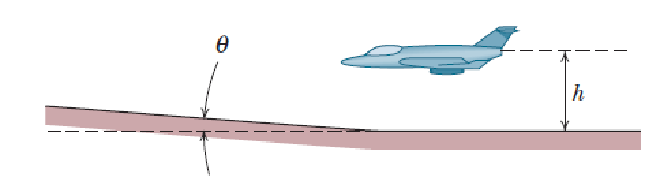
\includegraphics[scale=1.0]{Qfig3-2.pdf}  
  \caption{문제 1}
  \label{fig:1}
\end{figure} \\
\noindent {\bf 풀이}
전투기가 일정한 속도로 움직이고 있으므로 $t$초 동안 비행기가 움직인 거리는 속도와 시간의
곱으로 구할 수 있다.
\begin{align} \label{}
\ell = vt = (1300~\mathrm{km/h})t
\end{align}
전투기의 비행높이를 $h$라고 하면, $h$와 전투기가 이동한 거리 $\ell$의 관계식은 탄젠트 함수로 주어진다.
\begin{align} \label{}
\tan{\theta} = \frac{h}{\ell} = \frac{h}{vt}, \;\;\; \text{또는} \;\;\; t = 
\frac{h}{v\tan{\theta}}
\end{align}
경사면의 각도가 $4.3^\circ$이고 $h=3.5~\mathrm{m}$이므로 유효숫자를 고려하여 계산하면 다음과 같다.
\begin{align} \label{}
t &= \frac{(3.5~\mathrm{m})}{(1300~\mathrm{km/h})(\tan{4.3^\circ})} \cr
&= \frac{(3.5\times 10^{-3}~\mathrm{km})}{(1.3\times 10^3~\mathrm{km/h})(0.075)}
\cr
&= 3.6\times 10^{-4}~\mathrm{h} = (3.6\times 10^{-4}~\mathrm{h})
\frac{3600~\mathrm{s}}{1~\mathrm{h}} = 1.3~\mathrm{s}
\end{align}
즉 전투기는 약 $1.3$초 후 언덕과 충돌한다.
\begin{figure}[htp]
\centering
\includegraphics[scale=0.6]{QSfig3-1-20220307.png}
\caption{문제 2 풀이}
\end{figure}
\vspace{0.5cm}

\noindent {\bf 문제 4 [20pt]}
공사 중인 다리에서 볼트가 다리 아래 계곡으로 90 m 떨어진다.
\begin{itemize}
\item[(가)] 낙하거리의 마지막 20\% 지나는 데 걸리는 시간을 구하여라.
\item[(나)] 볼트가 낙하거리의 마지막 20\%를 들어설 때의 속력을
  구하여라.
\item[(다)] 다리 아래 계곡에 도달할 때 볼트의 속력을 구하여라.   
\end{itemize} 
\noindent {\bf 풀이}
(가) 초기 속도 $v_0=0$이므로, 볼트의 자유낙하는
\begin{align*}
y-y_0= -\frac12 gt^2  
\end{align*}
이 기술한다. $y_0=0$, $y=-90$ m이므로, $y-y_0=-90$ m이다. 볼트가
$y-y_0$의 80\%에 이르렀을 때 거리는 $(0.8)(-90)\, \mathrm{m}= -72$
m이므로  여기까지 도달하는 데 걸린 시간 $\tau$는 
\begin{align*}
-72\,\mathrm{m} = -\frac{g}{2} \tau^2  
\end{align*}
이 되고,
\begin{align*}
\tau = \sqrt{\frac{(2) (72\,\mathrm{m})}{9.8\,\mathrm{m/s^2}}} =
  3.83\,\mathrm{s} 
\end{align*}
이다. 그런데 -90 m 떨어지는 데까지 걸린 시간 $t$는
\begin{align*}
t = \sqrt{\frac{2(y_0-y)}{g}} = \sqrt{\frac{(2) (90\,\mathrm
  m)}{9.8\,\mathrm{m/s^2}}} = t = 4.29\,\mathrm{s}  
\end{align*}
이다. 따라서 볼트가 마지막 구간 20\%를 지나는 데 걸린 시간은
\begin{align*}
t' = t-\tau = (3.83-4.29)\,\mathrm{s} = 0.45\,\mathrm{s} 
\end{align*}
이다.
\\
\\
\noindent (나) 볼트가 마지막 남은 20\% 구간에 들어설 떄 속도 $v$는
\begin{align*}
\vec{v} = -g\tau\hat{\bm{j}} =
  -(9.80\,\mathrm{m/s^2})(3.83\,\mathrm{s})\hat{\bm{j}} \approx 
  38\,\mathrm{m/s}   \,\hat{\bm{j}}  
\end{align*}
가 되므로 속력은
\begin{align*}
  v = |\vec{v}| = 38\,\mathrm{m/s} 
\end{align*}
이다. 
\\
\\
\noindent (다)
마찬가지 방법으로 볼트가 바닥에 도달할 때 속도는 
\begin{align*}
  \vec{v}_f = -gt \hat{\bm{j}}  =
  -(9.80\,\mathrm{m/s^2})(4.29\,\mathrm{s}) \hat{\bm{j}}
  =-42\,\mathrm{m/s} \hat{\bm{j}}
\end{align*}
이고 속력은
\begin{align*}
v_f = |\vec{v}_f| = 42\, \mathrm{m/s}  
\end{align*}
가 된다.   

\end{document}
